\subsection{\stid{4} \dataviz}\label{subsect:dataviz}

\textbf{End State:} A production-quality storage infrastructure necessary to manage, share, and facilitate analysis of data in support of mission critical codes. Data analytics and visualization software that effectively supports scientific discovery and understanding of data produced by Exascale platforms.

\subsubsection{Scope and Requirements}
Changes in the hardware architecture of Exascale supercomputers will render current approaches to data management, analysis and visualization obsolete, resulting in disruptive changes to the scientific workflow and rendering traditional checkpoint/restart methods infeasible. A major concern is that Exascale system concurrency is expected to grow by five or six orders of magnitude, yet system memory and input/output (I/O) bandwidth/persistent capacity are only expected to grow by one and two orders of magnitude, respectively. The reduced memory footprint per FLOP further complicates these problems, as does the move to a hierarchical memory structure. Scientific workflow currently depends on exporting simulation data off the supercomputer to persistent storage for post-hoc analysis.

On Exascale systems, the power cost of data movement and the worsening I/O bottleneck will make it necessary for most simulation data to be analyzed in situ, or on the supercomputer while the simulation is running. Furthermore, to meet power consumption and data bandwidth constraints, it will be necessary to sharply reduce the volume of data moved on the machine and especially the data that are exported to persistent storage. The combination of sharp data reduction and new analysis approaches heighten the importance of capturing data provenance (i.e., the record of what has been done to data) to support validation of results and post-hoc data analysis and visualization.
Data and Visualization is the title for Data Management (DM) \& Data Analytics and Visualization (DAV) activities in the Exascale project.

Data management (DM) activities address the severe I/O bottleneck and challenges of data movement by providing and improving storage system software; workflow support including provenance capture; and methods of data collection, reduction, organization and discovery.

Data analytics and visualization (DAV) are capabilities that enable scientific knowledge discovery. Data analytics refers to the process of transforming data into an information-rich form via mathematical or computational algorithms to promote better understanding. Visualization refers to the process of transforming scientific simulation and experimental data into images to facilitate visual understanding. Data analytics and visualization have broad scope as an integral part of scientific simulations and experiments; they are also a distinct separate service for scientific discovery, presentation and documentation purposes, as well as other uses like code debugging, performance analysis, and optimization. 

The scope of activities falls into the following categories:
\begin{itemize}
\item Scalable storage software infrastructure – system software responsible for reliable storage and retrieval of data supporting checkpointing, data generation, and data analysis I/O workloads
\item Data collection, reduction, and transformation – enabling complex transformation and analysis of scientific data where it resides in the system and as part of data movement, in order to reduce the cost to solution
\item Data organization and discovery – indexing and reorganizing data so that relevant items can be identified in a time- and power-efficient manner, and complex scientific data analysis can be performed efficiently on Exascale datasets
\item In situ algorithms and infrastructure – performing DAV while data is still resident in memory as the simulation runs enabling automatic identification, selection and data reduction for Exascale applications.
\item Interactive post-hoc approaches – on data extracts that produced in situ and support post-hoc understanding through exploration.
\item Distributed memory multi-core and many-core approaches, for the portable, performant DM and DAV at Exascale.
\end{itemize}
\subsubsection{Assumptions and Feasibility}
\begin{itemize}
\item Scaling up traditional DM and DAV approaches is not a viable approach due to severe constraints on available memory and I/O capacity, as well as dramatically different processor and system architectures being at odds with contemporary DAV architectures.
\item Simulations will produce data that is larger and more complex, reflecting advances in the underlying physics and mathematical models. Science workflows will remain complex, and increasing requirements for repeatability of experiments, availability of data, and the need to find relevant data in Exascale datasets will merit advances in workflow and provenance capture and storage.
\item The expense of data movement (in time, energy, and dollars) will require data reduction methods, shipping functions to data, and placing functionality where data will ultimately reside.
\item Solid-state storage will become cheaper, denser, more reliable, and more ubiquitous (but not cheap enough to replace disk technology in the Exascale timeframe). Exascale compute environments will have in-system nonvolatile storage and off-system nonvolatile storage in addition to disk storage. Applications will need help to make use of the complex memory/storage architectures.
\item Disks will continue to gain density but not significant bandwidth; disks will become more of a capacity solution and even less a bandwidth one.
\item Industry will provide parts of the overall data management, data analysis and visualization solution, but not all of it; non-commercial parts will be produced and maintained.
\item This plan and associated costs were formulated based on the past decade of DOE visualization and data analysis activities, including the successful joint industry/laboratory-based development of open-source visualization libraries and packages (VTK, VisIt, and ParaView).
\end{itemize}
\subsubsection{Objectives}
Data management, analysis and visualization software must provide:
\begin{itemize}
\item production-grade Exascale storage infrastructure(s), from application interfaces to low-level storage organization, meeting requirements for performance, resilience, and management of complex Exascale storage hierarchies;
\item targeted research to develop a production-grade in situ workflow execution system, to be integrated with vendor resource management systems, meeting science team requirements for user-defined and system-provided provenance capture and retention;
\item production-grade system-wide data transfer and reduction algorithms and infrastructure, with user interface and infrastructure for moving/reducing data within the system, to be integrated with vendor system services and meeting science and national security team requirements; and
\item production-grade metadata management enabling application and system metadata capture, indexing, identification, and retrieval of subsets of data based on complex search criteria and ensures that technologies target science and national security team requirements.
\item targeted research to develop a production-grade in situ algorithms, to be integrated with open source visualization and analysis tools and infrastructure, meeting science team data reduction requirements
\item targeted research to develop a production-grade algorithms for the new types of data that will be generated and analyzed on Exascale platforms as a result of increased resolution, evolving scientific models and goals, and increased model and data complexity.
\item targeted research to develop a production-grade post-hoc approach that support interactive exploration and understanding of data extracts produced by in situ algorithms
\item production-grade Exascale data analysis and visualization algorithms and infrastructure, meeting requirements for performance, portability and sustainability for evolving hardware architectures and software environments. 
\end{itemize}

\subsubsection{Plan}
Productization of technologies is a necessary step for adoption, research-quality software is not enough. One approach we will take is to fund vendors of products in related areas to integrate specific technologies into their product line. When developing objectives for this activity, a focus was placed on the availability of products that deliver these technologies on platforms of interest. Activities can be separated into two categories:
\begin{itemize}
\item Community/Coordination – designed to build the R\&D community, inform ourselves and the community regarding activities in the area, track progress, and facilitate coordination.
\item Targeted R\&D – filling gaps in critical technology areas (storage infrastructure, workflow, provenance, data reduction and transformation, and organization and discovery).
\end{itemize}

Portions of the DAV software stack are being productized and supported by industry, which will help to control costs in the long term. Activities to achieve the DAV objectives are heavily dependent on developments across the Exascale project, and thus close coordination with other teams is essential. Close engagement with application scientists is crucial to the success of DAV, both in terms of understanding and addressing the requirements of science at scale and ensuring that computational scientists are able to adopt and benefit from the DAV deliverables.

Many objectives need initial research projects to define plausible solutions. These solutions will be evaluated and progressively winnowed to select the best approaches for the Exascale machine and the needs of science. Selected projects will continue to receive support to extend their research and development efforts to integrate their solutions into the open-source Exascale software stack. 

\subsubsection{Risks and Mitigations Strategies}
There are specific risks identified for the Data and Visualization portfolio.  These risks are tracked in the risk register .  
\begin{itemize}
\item Application teams may continue to employ ad hoc methods for performing data management in their work, resulting in increased I/O bottlenecks and power costs for data movement. Application team engagement, working within the overall software stack, and input into HI will be necessary if results are to be deployed, adopted, and significantly improve productivity.
\item Despite funding vendor activities, industry partners may determine the market is insufficient to warrant meeting Exascale requirements.
\item If vendor integration and targeted R\&D activities are not closely coordinated, gaps will not be effectively identified and targeted, or successful R\&D will not be integrated into industry products in the necessary timeframe.
\item Vendors supplying data management solutions are likely to be distinct from Exascale system vendors. Additional coordination will be necessary, beyond DM productization, in order to ensure interoperability of DM solutions with specific Exascale platforms.
\item Data management from an application perspective is tracked in one of the identified risks.  Additionally, the software stack tracks several risks indirectly related to data management as well.
\item Failure of scientists to adopt the new DAV software is a major risk that is exacerbated if the DAV software is research quality. Mitigating this risk depends on close engagement with domain scientists and supporting layers of the software stack through co-design activities, as well as investment in development and productization of DAV codes.
\item Redundant efforts in domain science communities and within ASCR-supported activities such as SciDAC result in wasted resources. Communication and close coordination provide the best strategy for mitigation.
\item Fierce industry and government competition for DAV experts creates a drain on laboratory personnel in DAV and makes lab hiring in this area difficult. Stable funding and a workforce development program would help to mitigate these risks.
\item A skilled workforce is required for a successful Exascale project.
\end{itemize}

\subsubsection{Future Trends}

\textbf{Graphics Architectures and Approaches}  Graphics architectures are improving in terms of raw computational power and through the addition of specialized libraries for accelerating ray-tracing, volume rendering, and denoising. Nvidia has added specialized hardware processing units for ray-tracing and machine learning to their GPU offerings.  Intel has developed a suite of CPU accelerated libraries that support OpenGL (OpenSWR), ray-tracing (Embree, OSPRay), volume rendering (Open Volume Kernel Library) and de-noising (Open Image Denoise). From a visualization and rendering perspective, ray-tracing provides significantly improved rendered results over traditional scan-conversion based approaches.  A near-term opportunity is to take advantages of such functionality for our rendering needs. Longer term, we will look into leveraging these hardware accelerated approaches to accelerate visualization and analysis tasks.

\textbf{In Situ Analysis and Automation}  A key thrust of the Data and Visualization area is the focus on in situ analysis in order to filter important information as it is being generated by the simulations. In addition to our algorithmic and infrastructure efforts, automatic techniques and workflows must be developed to guide the overall in situ analysis process.

\textbf{Workflows} Slowly, more complex workflows are becoming a more significant component of the job mix on ECP-relevant platforms, partially driven by the increased use of these systems for machine learning applications. Workflows can drive degenerate use cases in the storage stack, such as the use of the file system for communication between tasks, when tools from outside the HPC community are adopted without change. Alternative approaches to enable communication between tasks exist but must be adapted to facility contexts, and technical roadblocks (e.g., difficulty in communicating between separate jobs) must be overcome.

\textbf{AI} AI applications will appear more frequently in the job mix. This impacts the requirements for data storage, as new classes of data become more prominent in application input datasets. It also impacts technologies for understanding application behavior, as these jobs are often not using MPI, a common assumption in tool sets. Finally AI-focused applications do not exhibit the common pattern of alternating phases of I/O and computation seen in simulation codes, driving a need for attention on methods of I/O optimization that do not rely on explicit collective I/O phases.

\textbf{Networks} Network architectures are still in flux, and specific new technologies such as Slingshot from Cray will bring new capabilities such as more advanced congestion detection and mitigation that change how networks will behave in the face of mixed communication and I/O traffic or the impact of communication-heavy applications on other applications in the system, etc.  Assumptions regarding how I/O traffic fits into this picture may need to be reexamined. The libfabric interface for accessing networks appears to be the most promising portable interface for use outside of MPI, and teams will need to assess how to best use libfabric across platforms of interest as well as possibly advocating for specific capabilities in libfabric that fall outside of traditional MPI use cases, such as the common pattern of clients connecting and detaching from long-running services.

\textbf{Object stores} Facilities are planning deployments of non-POSIX storage solutions. One of the first of these will be the DAOS deployment on the A21 system at Argonne. The DAOS interfaces are available for teams to begin to understand, an HDF5 front-end for DAOS is available, and there are some examples of DAOS use for scientific codes. It is likely that the highest performance will come from applications directly using the DAOS APIs, and work to allow understanding of how these APIs are used would be beneficial.

\textbf{Compression} Compression will continue to play an important role in computation as a vehicle for addressing the explosion in size of datasets and outputs. Improved integration of compression capabilities in libraries supporting parallel I/O will continue to be a topic for further development, and techniques for allowing concurrent updates while compression is enabled specifically need more exploration.  The use of lower precision data types has the potential of speeding up the visualization and analysis process as well as reducing data sizes without significantly degrading the accuracy of results. 

\textbf{Storage technologies and architectures} Even in systems that will continue to employ POSIX file systems as the main "scratch" store, the hardware on which these file systems are stored will be changing. For example, the Perlmutter system will provide a 30~PB nonvolatile storage tier using Lustre. The file system teams (e.g., Lustre team) will be working to maximize performance on these new storage back-ends, but simultaneously higher software layers must consider how this significant change impacts their assumptions about the relative costs of communication and data storage for common patterns of access.


% STORAGE ARCH. DIAGRAM -- HIGH LEVEL
\begin{figure}[htb!]
	\centering
	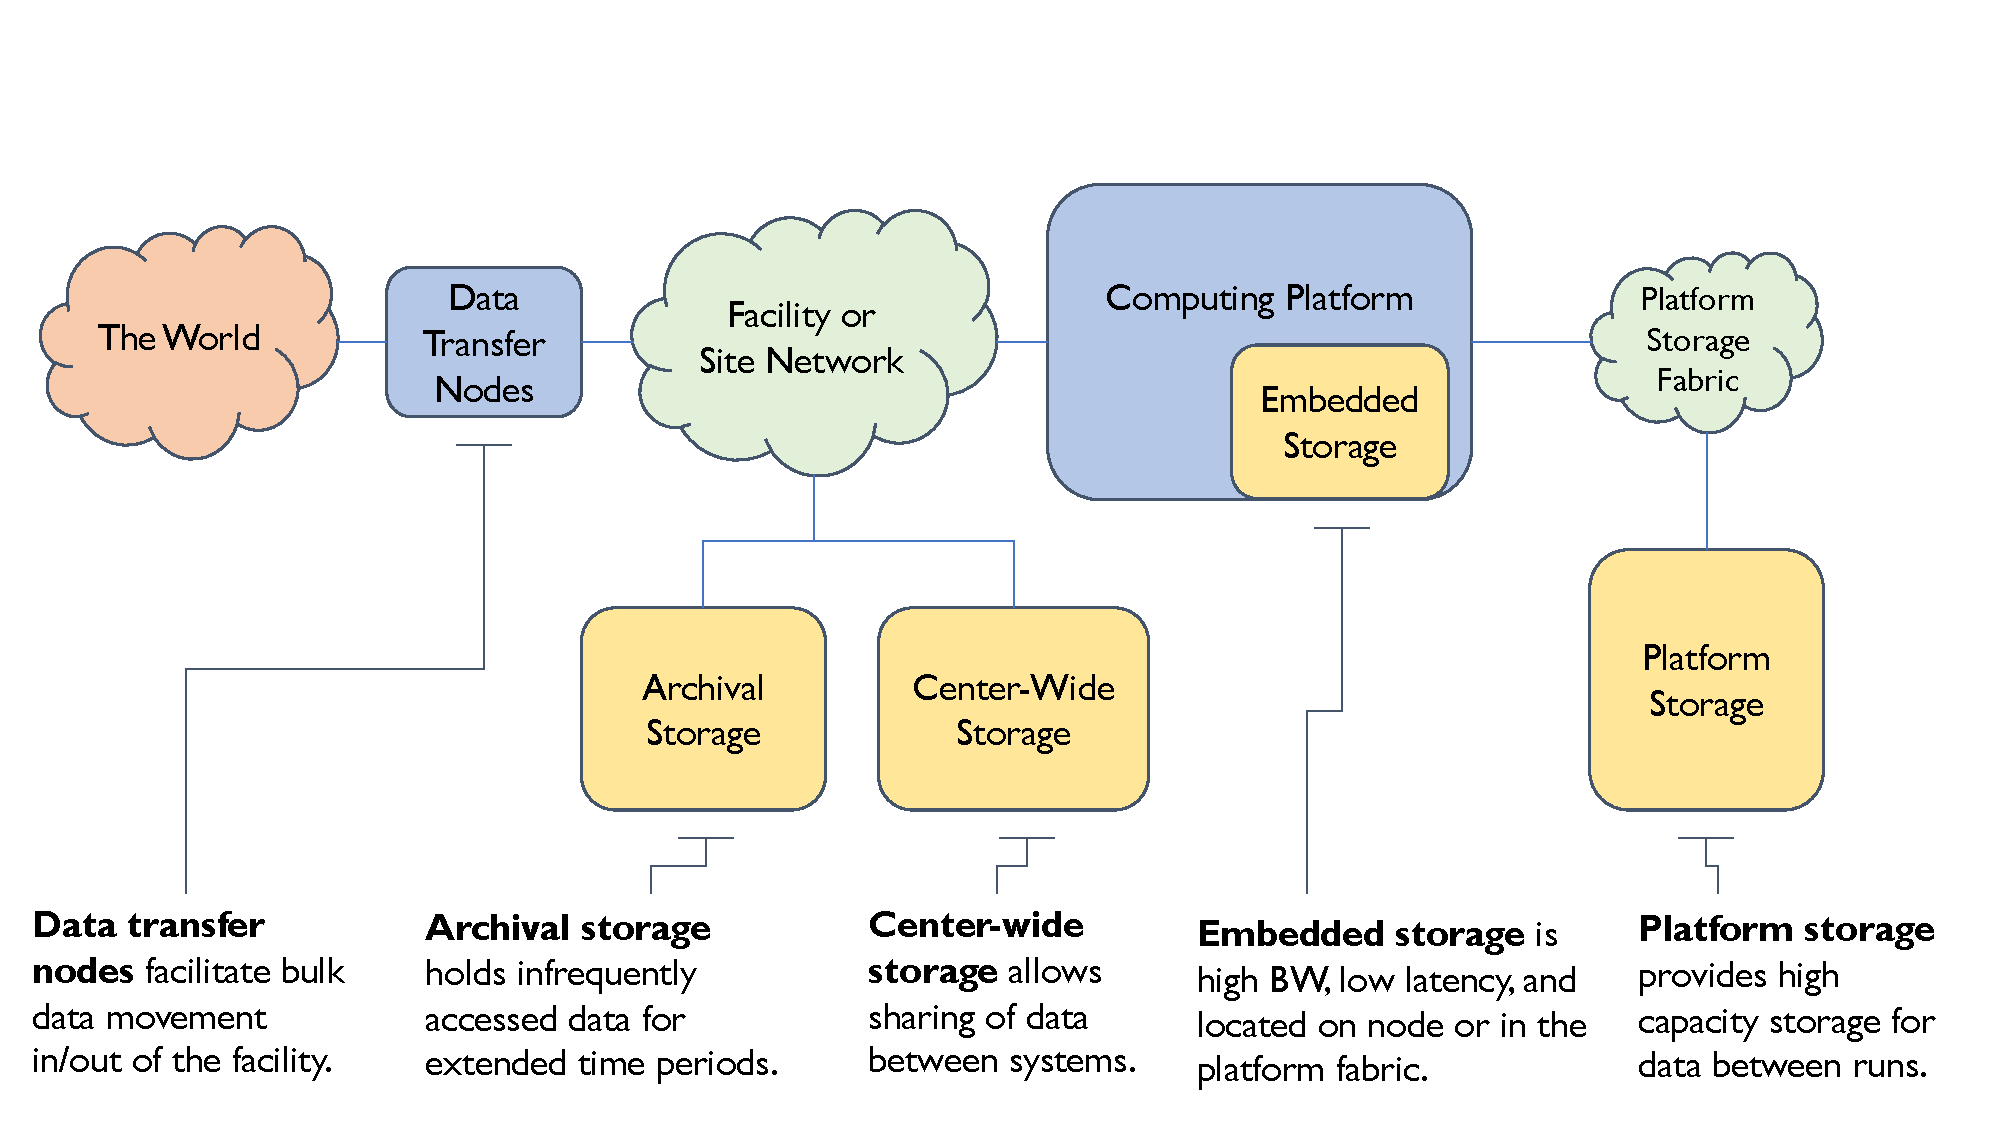
\includegraphics[width=0.70\textwidth]{projects/2.3.4-DataViz/DataViz-storage-notional-diagram.pdf}
	\caption{\label{fig:DataViz:StorageDiagram} A notional diagram of DOE
		facility storage resources. Not all systems have each role filled,
		and often additional network connections exist to accelerate specific
		data flows.}
\end{figure}


% FUTURE: STORAGE TECHNOLOGIES AND ARCHITECTURES
Figure~\ref{fig:DataViz:StorageDiagram} depicts a notional diagram of
the storage resources surrounding a leadership class platform at a DOE
facility. In this diagram, ``platform'' is the HPC system itself: Theta, Summit,
Cori, Frontier, Perlmutter, Aurora, etc. 

Note that this is a notional diagram. There are often additional
connections to speed specific transfers, and some sites augment one resource
while omitting another.
%
Data transfer nodes provide access to data stored on facility storage from the
outside world: Typically this is enabled using GridFTP, Globus Online, htar, or
similar.

There are lots of roles that storage might play:
\begin{itemize}
	\item \emph{Archival storage} holds ``cold'' data. Currently tape is
	still the dominant media for archival storage, but disk is also used,
	both as cache and as permanent storage (sometimes spun down).
	\item \emph{Center-wide storage} allows for easy data access between
	systems. This might include home directories and some other shared data
	volumes. Often performance is limited compared to platform storage.
	\item \emph{Platform storage} is storage that is connected to a limited
	number of platforms in the facility and is meant to be a high-performance,
	high-capacity store for data that will be used for multiple runs. While
	disk drives are still used in some platform storage deployments,
	increasingly solid-state storage (e.g., SSDs) is being employed in
	this role.
	\item \emph{Embedded storage} is located very close to the platform
	itself, either as node-local storage or tightly integrated into the
	fabric. Technologies used include NVMe and SSDs. Embedded storage that
	is available across the system is perhaps best thought of as a special 
	kind of platform storage.
\end{itemize}

%
% CURRENT STORAGE SPECS
%
\begin{table}[htb!]
	\vspace{-2mm}
	\centering
	\caption{\label{table:DataViz:StorageSpecsCurrent} Storage system specifications for current platforms.}
	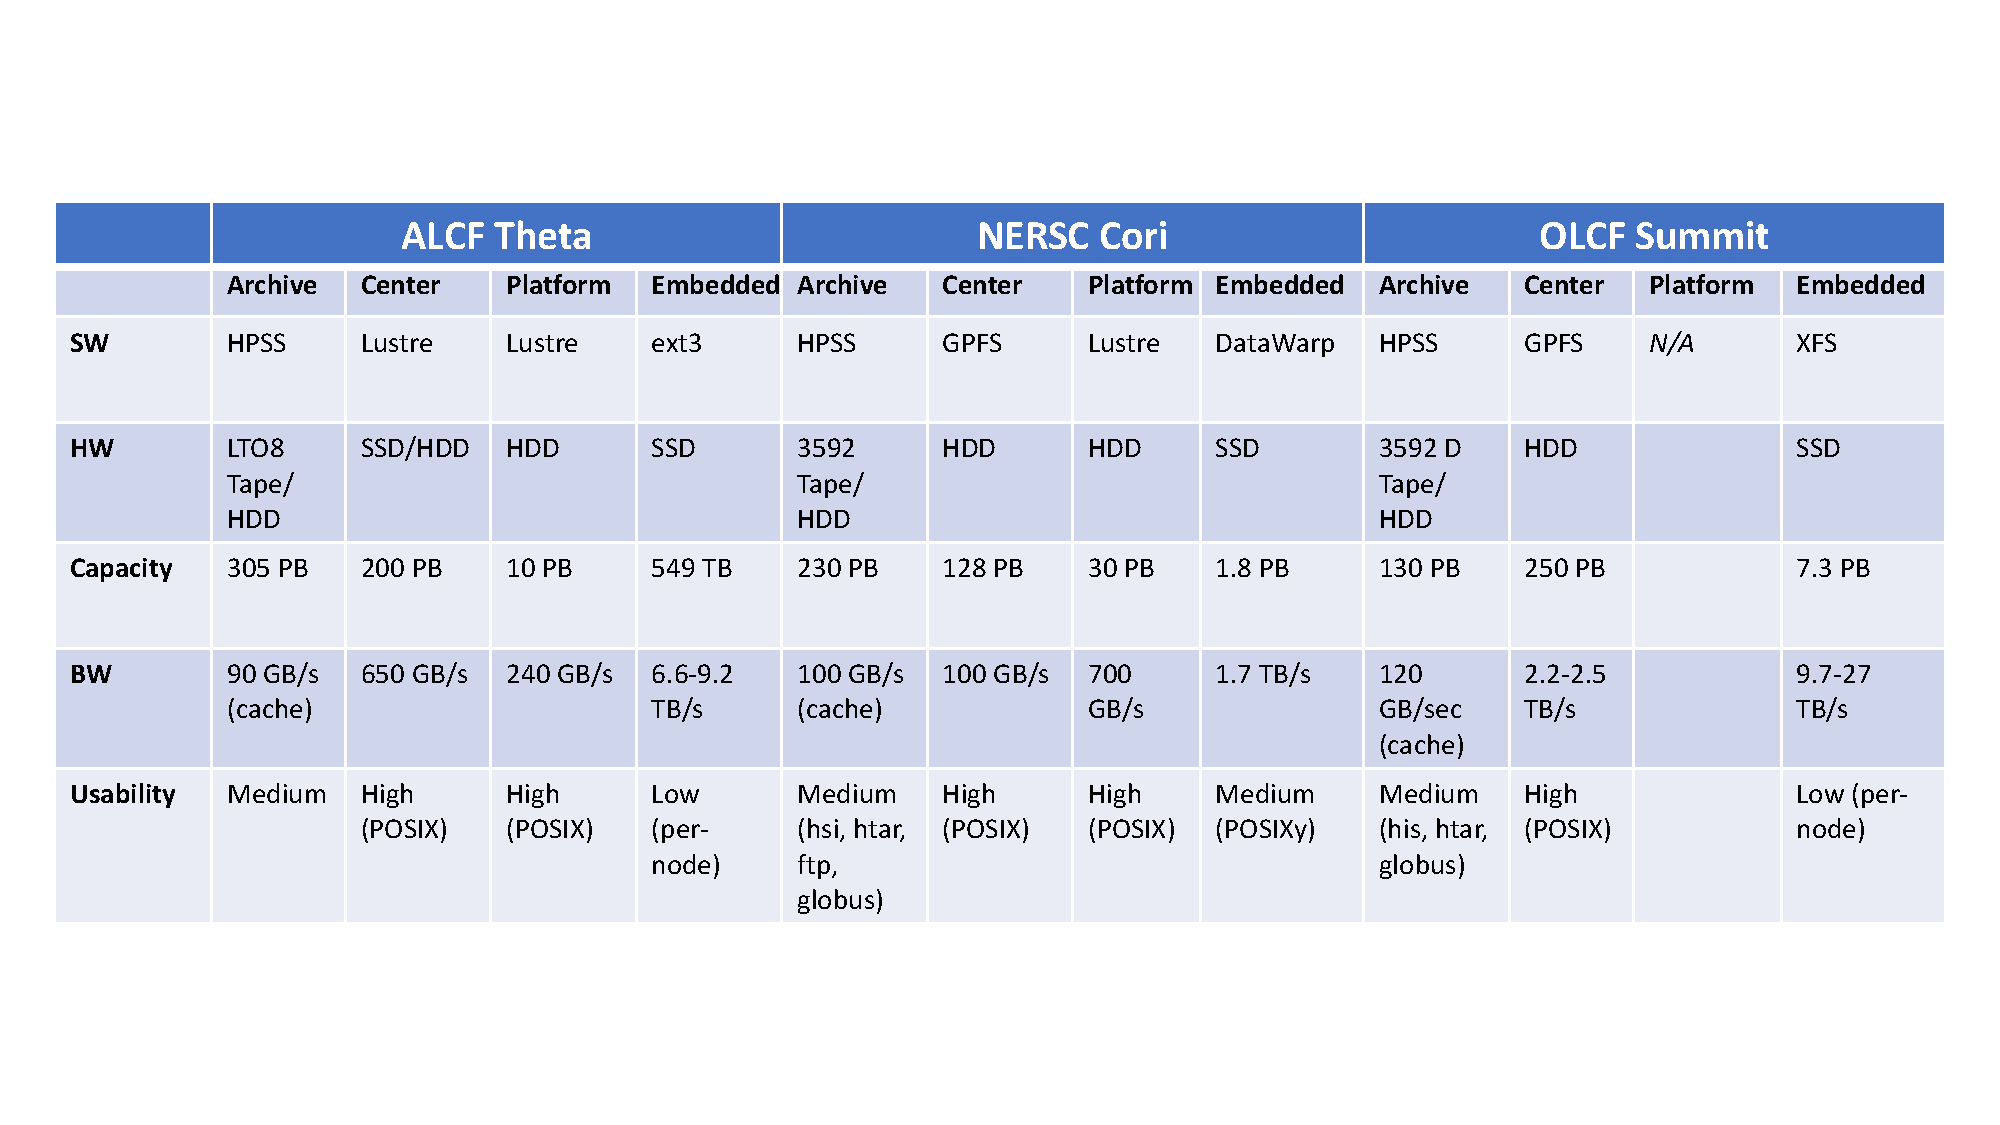
\includegraphics[width=0.75\textwidth]{projects/2.3.4-DataViz/DataViz-storage-specs-current.pdf}
\end{table}

Table~\ref{table:DataViz:StorageSpecsCurrent} captures the salient
characteristics of the storage deployments for the current generation of
systems: Theta, Cori, and Summit. These systems largely reflect trends in DOE
storage over the last decade: HPSS archival storage coupled with a POSIX
center-wide file system provided by GPFS or Lustre and backed by hard disk
drives (HDDs). In two cases, a faster, platform-specific POSIX file system is 
deployed, while at OLCF the team chose to instead concentrate on a very high
performance center-wide file system that is available on other resources as well.

Of note in these systems are some embedded storage options that have
provided the community with some early experiences with SSD storage. On
Theta and Summit, local SSDs are available that have seen limited use
by specific teams. On Cori, the DataWarp service allows for SSD-backed
storage pools to be allocated that are visible to an entire job or
workflow. This functionality is close to the model that users are
accustomed to, and the resource has seen significant use.

%
% PROJECTED FUTURE SPECS
%
\begin{table}[htb!]
	\vspace{-2mm}
	\centering
	\caption{\label{table:DataViz:StorageSpecsNext} Projected storage specifications for upcoming platforms.}
	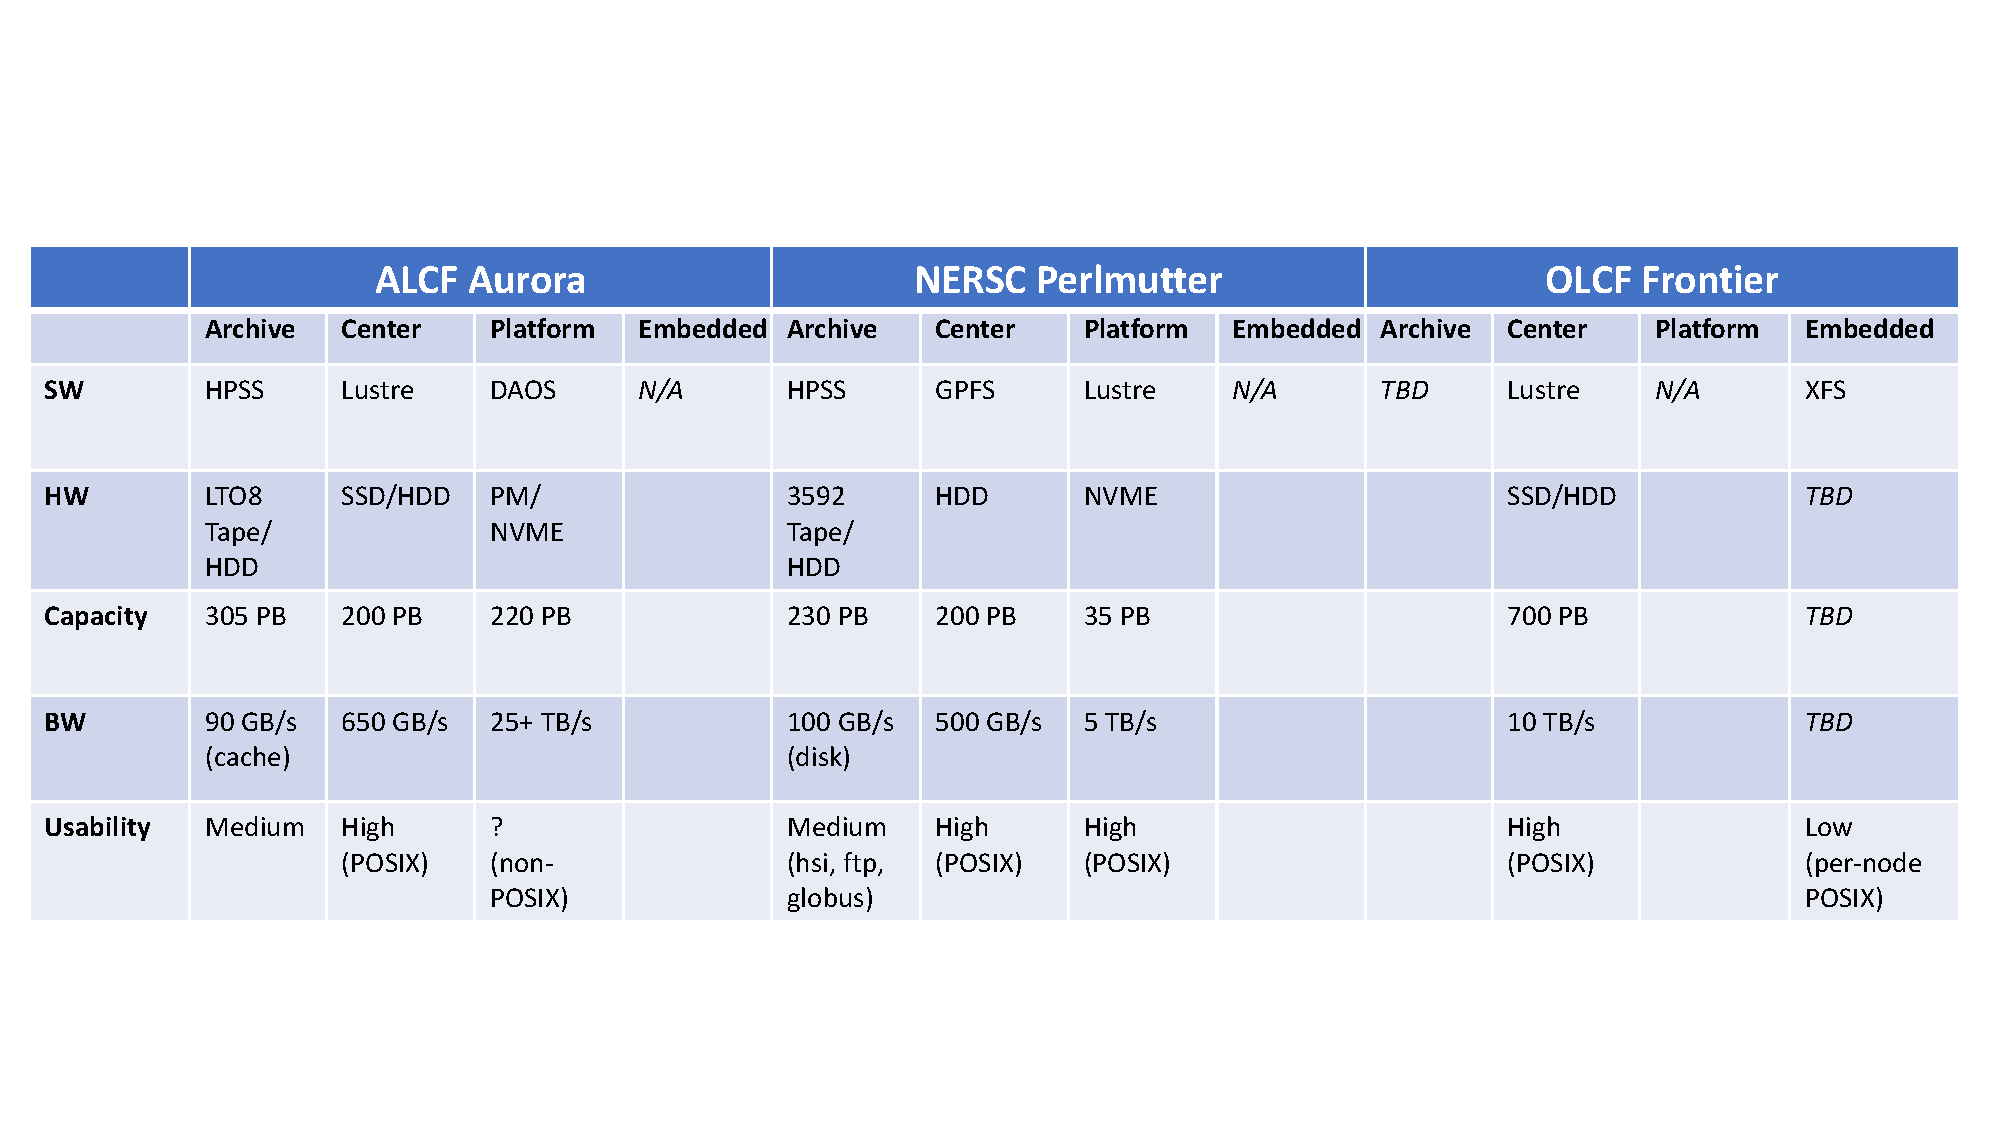
\includegraphics[width=0.75\textwidth]{projects/2.3.4-DataViz/DataViz-storage-specs-next.pdf}
\end{table}

Table~\ref{table:DataViz:StorageSpecsNext} captures the current, public
understanding of storage characteristics for the next generation of
systems: Aurora, Perlmutter, and Frontier.
%
A number of observations can be made from this data. First, POSIX will
remain the dominant (at least low-level) API for interacting with the primary
storage resources (embedded, platform, and center-wide). Obtaining peak
performance will likely remain a challenge for users, but with node counts
somewhat stalled, storage software scalability is not further pressured.
%
Second, DAOS, will appear as a POSIX alternative. DAOS is an Intel
product that will provide a form of globally accessible key-value
style of storage. However, a POSIX ``veneer'', or compatibility layer,
will be provided that will give users an easy way to make use of the
resource. With all the major ST I/O libraries already having the ability
to implement alternative back-ends, 
the challenge will be more about how to persist things \emph{outside} DAOS efficiently (e.g., converting back
to POSIX files).
%
Finally, there will still be a non-global, embedded storage resource on
Frontier. The best ways to utilize this resource need to be studied, but systems
like UnifyFS could play a role.

